%%%%%%%%%%%%%%%%%%%%%%%%%%%%%%  IEEEsample.tex  %%%%%%%%%%%%%%%%%%%%%%%%%%%%%%%
%%%%%%%%%%                                                        %%%%%%%%%%%%%
%%%%%%%%%%    More information: see the header of IEEEtran.sty    %%%%%%%%%%%%%
%%%%%%%%%%                                                        %%%%%%%%%%%%%
%%%%%%%%%%%%%%%%%%%%%%%%%%%%%%%%%%%%%%%%%%%%%%%%%%%%%%%%%%%%%%%%%%%%%%%%%%%%%%%
%
%\documentstyle[twocolumn]{IEEEtran}

%\documentclass[a4paper]{article}

% The amsmath and epsfig packages greatly simplify the process of adding
% equations and figures to the document, and thus their use is highly
% recommended.
% ------------

\documentclass[10pt,conference,a4paper]{IEEEtran}


\usepackage{amsmath}
\usepackage{epsfig}
\usepackage{graphicx}
\usepackage{acronym}
\usepackage{array}
\usepackage{listings}
\usepackage[latin1]{inputenc}
\usepackage{amsmath}
\usepackage{amsfonts}
\usepackage{amssymb}
\usepackage{graphicx} 
\usepackage[latin1]{inputenc}
\usepackage{amsmath}
\usepackage{amsfonts}
\usepackage{amssymb}  
\usepackage{fancyhdr}
\usepackage{listings}
\usepackage{url}
\usepackage{float}

\usepackage{acronym}
\usepackage{caption}
\usepackage{subcaption}
\usepackage{setspace}
\usepackage{underlin}
\usepackage{algpseudocode}
\usepackage{algorithm}
\usepackage{amssymb}
\usepackage{booktabs}
\usepackage{makeidx} 
\usepackage{microtype} 


\newcommand{\HRule}{\rule{\linewidth}{0.5mm}}

\acrodef{fpga}[FPGA]{Field programmable gate array}
\acrodef{cpld}[CPLD]{complex programmable logic device}
\acrodef{asic}[ASIC]{application specific integrated circuits}
\acrodef{isa}[ISA]{instruction set architecture}
\acrodef{gpu}[GPU]{graphic processing unit}
\acrodef{fpu}[FPU]{floating processing unit}
\acrodef{hdl}[HDL]{hardware description language}
\acrodef{api}[API]{application programming interface}
\acrodef{ip}[IP]{intellectual property}
\acrodef{lut}[LUT]{lookup tables}
\acrodef{bram}[BRAM]{block RAM}
\acrodef{dsu}[DSU]{debug support unit}
\acrodef{alu}[ALU]{arithmetic logical unit}
\acrodef{cam}[CAM]{custom address memory}
\acrodef{hll}[HLL]{higher level languages}
\acrodef{cpu}[CPU]{central processing unit}
\acrodef{par}[PAR]{place and route}
\acrodef{ai}[AI]{artificial intelligence}
\acrodef{ipc}[IPC]{instruction per cycle}
\acrodef{fd}[FD]{finite difference}
\acrodef{ea}[EA]{evolutionary algorithms}
\acrodef{ann}[ANN]{artificial neural network}
\acrodef{svm}[SVM]{support vector machines}
\acrodef{veb}[VEB]{virtual embedded block}
\acrodef{mmu}[MMU]{Memory Management Unit}
\acrodef{cpld}[CPLD]{complex programmable logic device}
\acrodef{asic}[ASIC]{application specific integrated circuits}
\acrodef{isa}[ISA]{instruction set architecture}
\acrodef{gpu}[GPU]{graphic processing unit}
\acrodef{fpu}[FPU]{floating processing unit}
\acrodef{hdl}[HDL]{hardware description language}
\acrodef{api}[API]{application programming interface}
\acrodef{ip}[IP]{intellectual property}
\acrodef{lut}[LUT]{lookup tables}
\acrodef{bram}[BRAM]{block RAM}
\acrodef{dsu}[DSU]{debug support unit}
\acrodef{alu}[ALU]{arithmetic logical unit}
\acrodef{cam}[CAM]{custom address memory}
\acrodef{hll}[HLL]{higher level languages}
\acrodef{cpu}[CPU]{central processing unit}
\acrodef{par}[PAR]{place and route}
\acrodef{ai}[AI]{artificial intelligence}
\acrodef{ipc}[IPC]{instruction per cycle}
\acrodef{fd}[FD]{finite difference}
\acrodef{ea}[EA]{evolutionary algorithms}
\acrodef{ann}[ANN]{artificial neural network}
\acrodef{svm}[SVM]{support vector machines}
\acrodef{veb}[VEB]{virtual embedded block}
\acrodef{mmu}[MMU]{Memory Management Unit}
\acrodef{rmt}[RMT]{remapping table}
\acrodef{lnreg}[LNreg]{Line Number Register}
\acrodef{secrand}[SecRAND]{Security-Aware Random Replacement Algorithm}
\acrodef{aes}[AES]{Advanced Encryption System}
\acrodef{asi}[ASI]{Address space identifier}
\acrodef{fsm}[FSM]{Finite State Machines}
\acrodef{pca}[PCA]{Principal Component Analysis}
\acrodef{asip}[ASIP]{Application Specific Instruction Processor}
\acrodef{gp}[GP]{Gaussian Process}
\acrodef{gbsa}[GbSA]{Galaxy-based Search Algorithm}
\acrodef{aco}[ACO]{Ant Colony Optimization}
\acrodef{pso}[PSO]{Particle Swarm Optimization}
\acrodef{sa}[SA]{Simulated Annealing}
\acrodef{ga}[GA]{Genetic Algorithm}
\acrodef{iwdp}[IWDP]{Intelligent Water Drops}
\acrodef{hpc}[HPC]{High Performance Computing}
\acrodef{ib}[IB]{Investment Banking}
\acrodef{par}[PAR]{Place and Route}
\acrodef{agppso}[A-GP-PSO]{Adaptive Gaussian Process Particle Swarm Optimizer}
\acrodef{vpso}[VPSO]{Adaptive Velocity Particle Swarm Algorithm}
\acrodef{aes}[AES]{Advanced Encryption System}
\acrodef{cad}[CAD]{Computer Aided Design}
\acrodef{svm}[SVM]{Support Vector Machine}
\acrodef{alo}[MLO]{Machine Learning Optimizer}
\acrodef{rvm}[RVM]{Relevance Vector Machine}
\acrodef{rbf}[RBF]{Radial Basis Function}
\newcommand{\ra}[1]{\renewcommand{\arraystretch}{#1}}


\pagestyle{headings}

\begin{document}

%\mainmatter  % start of an individual contribution

\title{Multi-objective Optimization of Parametric Reconfigurable Designs Using Machine Learning Optimizer}

% a short form should be given in case it is too long for the running head

% the name(s) of the author(s) follow(s) next
%
% NB: Chinese authors should write their first names(s) in front of
% their surnames. This ensures that the names appear correctly in
% the running heads and the author index.
%
\author{Maciej Kurek \and Tobias Becker \and Wayne Luk}
%
%\authorrunning{M. Kurek, T. Becker and W. Luk}
% (feature abused for this document to repeat the title also on left hand pages)

% the affiliations are given next; don't give your e-mail address
% unless you accept that it will be published
%\institute{Department of Computing, Imperial College London}

%\toctitle{Lecture Notes in Computer Science}
%\tocauthor{Authors' Instructions}
\maketitle


\begin{abstract}

This paper presents an enhancement of a novel technique that uses meta-heuristics and machine learning to automate the optimization of design parameters for reconfigurable designs. We previously developed \ac{alo} which from a number of benchmark executions automatically derive the characteristics of the parameter space and creates a surrogate model through regression and classification. Based on this surrogate model, design parameters are optimized with meta-heuristics. We present a new multi-objective flavor of the \ac{alo}. We evaluate the extended algorithm using two applications as well as investing \ac{fpga} architecture exploration. 

\end{abstract}

\section{Introduction}

We shown it to be useful to construct surrogate models of fitness functions representing design quality of reconfigurable hardware designs \cite{fpt2012MLO,arc2012MLO}. As these models are orders of magnitude faster to evaluate than the actual benchmarks and bitstreams, they can substantially accelerate optimization thus allowing for an automated approach. This is the motivation behind our development of the \ac{alo} tool which we apply to the problem of reconfigurable designs parameter optimization. Recently however; issues like power efficiency or size have become more prominent, expanding the problem into the multi-objective optimization domain. We present a new multi-objective flavor of \ac{alo} and evaluate it using a number of examples. The contributions of this paper are: 

\begin{list}{$\bullet$}{\itemsep 0.5ex}

\item A mathematical characterization of multi-objective optimization in reconfigurable applications. We extend the previous description \cite{arc2012MLO} (Section \ref{design}).

\item A new multi-objective version of \ac{alo}. We show how multiple Bayesian regressors and multi-objective meta-heuristics can be interlinked (Section \ref{surrogatemodels}).

\item An evaluation of the extended \ac{alo} approach using thre case studies: (a) a previously used \cite{fpt2012MLO} throughput of a quadrature based financial application with varied precision (Section \ref{evaluation}), and (b) and .
\end{list}


\section{Background}

\acp{fpga} allow designs that are customized to the requirement of the application, designers are often confronted with a very large parameter space. As a result the parameter space exploration can take an immense amount of time. A number of researchers approach the problem of high-cost fitness functions and large design spaces in various fields \cite{1041556,surrogateModel,Su:2008:GPA:1494644.1494688,5194095,LeThi2002258} by having fitness functions combined with fast-to-compute surrogate models provided by a \ac{gp} for decreasing evaluation time. However most current surrogate models only consist of a regressor and do not take into account possible invalid configurations within the design space. Eliminating regions producing invalid designs trims the design space, substantially reducing the complexity of the problem.


The reconfigurability and customization of \ac{fpga} designs potentially increases performance and efficiency. Unfortunately, the optimization of reconfigurable designs often requires substantial effort from designers who have to analyze the application, create models and benchmarks and subsequently use them to optimize the design. This process often involves adjusting multiple design parameters such as numerical precision, degree of pipelining or number of cores. One could proceed with automated optimization based on an exhaustive search through design parameters which are derived from application benchmarks; however, this is unrealistic since benchmark evaluations involve bitstream generation and code execution which often takes hours of compute time. Surrogate models approximating fitness functions by substituting lengthy evaluations with estimations based on closeness in a design space have been investigated in reconfigurable computing \cite{Pilato2008}. The work covers surrogate models for circuit synthesis from \ac{hll}, rather than parameter optimization.

%\subsection{Gaussian Process Regression}

\ac{gp} is a machine learning technology based on strict theoretical fundamentals and Bayesian theory \cite{Seeger04gaussianprocesses,Rasmussen06gaussianprocesses}. \ac{gp} does not require a predefined structure, can approximate arbitrary function landscapes including discontinuities, and includes a theoretical framework for obtaining the optimum hyper-parameters \cite{5194095}. An advantage of \ac{gp} is that it provides a predictive distribution, not a point estimate.

 %can have meaningful hyper-parameters,%

A Gaussian process is a collection of random variables, any finite set of which have a joint Gaussian distribution. A Gaussian process is completely specified by its mean function $m(\mathbf{x})$ and the covariance (kernel) function $k(\mathbf{x},\mathbf{x'})$:

%\vspace{-1em}


\begin{align} 
\hat{f}(\mathbf{x}) \sim \mathcal{G}\mathcal{P}(m(\mathbf{x}),k(\mathbf{x},\mathbf{x'}))
\end{align}

%\vspace{-0.5em}

The $k(\mathbf{x},\mathbf{x'})$ expresses the covariance between pairs of random variables, and in regression analysis it expresses the relation between input-output pairs. This is based on a training set $\mathcal{D}$ of $n$ observations, $\mathcal{D}={(\mathbf{x}_i,y_{i}) | i = 1, ... n} $, where $\mathbf{x}$ denotes an input vector, $y$ denotes a scalar output. The column vector inputs for all $n$ cases are aggregated in the $D \times n$ design matrix $X$, and the outputs are collected in the vector $\mathbf{y}$. The goal of Bayesian forecasting is to compute the distribution $p(\hat{f}|\mathbf{x_*},\mathbf{y},X)$ of the function $\hat{f}$ at unseen input $\mathbf{x_{*}}$ given a set of training points $\mathcal{D}$. Using Bayes rule, the predictive posterior for the Gaussian process $\hat{f}$ and the predicted scalar outputs $\hat{f}(\mathbf{x_*})=y_*$ can be obtained.

% By conditioning on the observed targets in the training set, the predictive distribution is Gaussian.

%\vspace{-1em}


%\subsection{Support Vector Machines Classification}

\ac{svm} is a maximum margin classifier, which constructs a hyperplane used for classification (or regression) \cite{Bishop:2006:PRM:1162264}. \acp{svm} use kernel functions $k(\mathbf{x},\mathbf{x'})$ to transform the original feature space to a different space where a linear model is used for classification. \acp{svm} are a class of decision machines and so do not provide posterior probabilities. There is a training set $\mathcal{D}$ of $n$ observations, $\mathcal{D}={(\mathbf{x}_i,t_{i}) | i = 1, ... n} $, where $\mathbf{x}$ denotes an input vector, $t$ denotes a target value. The column vector inputs for all $n$ cases are aggregated in the $D \times n$ design matrix $X$, and the targets in the vector $\mathbf{t}$. The goal is to classify an unseen input $\mathbf{x_{*}}$ based on $X$ and $\mathbf{t}$ by computing a decision boundary. 

%\begin{align} 
%f(x) = w^{T} \phi(x) + \beta
%\end{align}

%\vspace{-1em}


%\subsection{Particle Swarm Algorithm (PSO)}
%with inertia governing its movement
\ac{pso} is a population-based meta-heuristic based on the simulation of the social behavior of birds within a flock \cite{VanDenBergh:2002:APS:935867}. The algorithm starts by randomly initializing $N$ particles where each individual is a point in the $\mathcal{X} = \mathbb{R} \times ... \times \mathbb{R}$ search space. The population is updated in an iterative manner where each particle is displaced based on its velocity $v_{id}$. The criteria for termination of the \ac{pso} algorithm can vary, and usually are determined by a time budget. The $x_{id}$ represents the $d$th coordinate of particle $i$ from the set $X_*$ of $N$ particles, where particle is a point within $\mathcal{X}$. In the most basic form of \ac{pso} Eq. \ref{eq:pso1}-\ref{eq:pso2} govern movement of particles. $r_1 \sim U(0,1)$ and $r_2 \sim U(0,1)$ are two independent uniformly distributed random numbers, $c_1$ and $c_2$ are acceleration coefficients and $p_{gd}$ and $p_{id}$ are $d$th coordinates of the global best and personal best positions. $p_{gd}$ is updated when a new global best fitness is found and $p_{id}$ is updated when a particle improves over its best fitness.

%\vspace{-1.5em}


\begin{align} 
\label{eq:pso1}
v_{id}=v_{id}+c_{1}r_{1}(p_{id}-x_{id}) + c_{2}r_{2}(p_{gd}-x_{id})
\end{align}

%\vspace{-2.5em}


\begin{align} 
\label{eq:pso2}
x_{id}=x_{id}+v_{id} 
\end{align}

%\vspace{-1.9em}


\section{Optimization Approach} 
\label{design}
%y fitness function of a heterogeneous application we understand fitness provided by execution of the applications benchmark.
%The challenge we address is encapsulation of reconfigurable designs $\mathcal{X}$ to provide an environment suitable for meta-heuristic to minimize benchmark evaluations. 
% If the optimizer fails to deliver optimal value, we have to increase its time and resource budget or re-design the application.

Traditionally, optimization of reconfigurable applications is carried out by building benchmarks and relevant tools, and the associated analytical models \cite{Anson2012Quad,Becker:2009:PDR:1530588.1530595}. This involves the following steps:

%\vspace{-0.5em}

\begin{enumerate}\addtolength{\itemsep}{-0.1\baselineskip}  
\item Build application and a benchmark returning design quality metrics.
\item Specify search space boundaries and optimization goal.
\item Create analytical models for the design.
\item Create tools to explore the parameter space.
\item Use the tools to find optimal configurations, guided by the models in step 3.
\item If result is not satisfactory, redesign.
\end{enumerate}

%\vspace{-0.5em}

In our approach the user supplies a benchmark along with constraints and goals, and the MLO automatically carries out the optimization (Algorithm \ref{ourmlo}). Our approach consists of the following steps:

\begin{enumerate}\addtolength{\itemsep}{-0.1\baselineskip}  
\item Build application and benchmark returning design quality metrics.
\item Specify search space boundaries and optimization goal.
\item Automatically optimize design with \ac{alo}.
\item If result is not satisfactory, redesign or revised time budget and search space.

\end{enumerate}

Our idea of surrogate modeling is illustrated in Fig.~\ref{fig:ouridea}. The \ac{alo} algorithm explores the parameter space by evaluating different benchmark configurations as presented in the left figure. The results obtained during evaluations are used to build a surrogate model which provides a regression of the fitness function and identifies invalid regions of the parameter space. A meta-heuristic (currently \ac{pso}) guides the exploration of the parameter space using the surrogate model. 

%Our steps 1, 2 and 4 correspond to traditional steps 1, 2 and 6. Therefore our approach is faster than the traditional
%approach if the time taken during our step 3 is shorter than the total time taken for steps 3, 4 and 5 of the traditional approach. Our approach will get faster the less time individual steps take. 

%We contrast two approaches in Fig.~\ref{fig:ouridea}.

  \begin{figure*}
     \centering
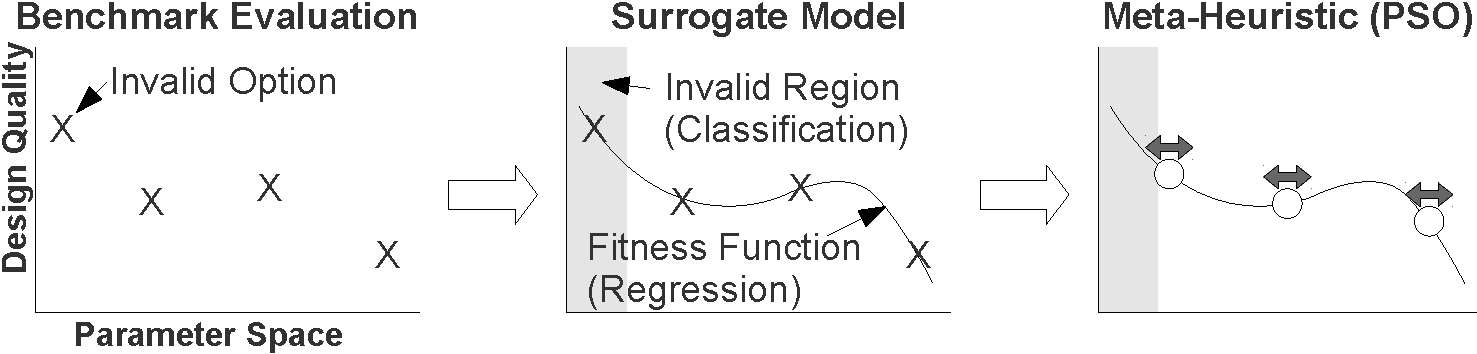
\includegraphics[width=1.0\textwidth]{./graphics/surrogate_tobias.pdf}
        \caption{Benchmark evaluations, surrogate model and model guided search.}     
           \label{fig:ouridea}
  \end{figure*}
 
%We use meta-heuristics to explore parameter space. The challenge with applying meta-heuristics to reconfigurable design parameter optimization is related to high cost of fitness function evaluations (application benchmark evaluations). Our proposed optimization approach has three new aspects that counter this problem. We define a mathematical description of reconfigurable designs parameter space and provide a formal definition of the fitness function based on application benchmarks and the parameter space (Section \ref{designspace} and \ref{fitfunction})). By doing so we provide an environment suitable for meta-heuristic optimization. Using the defined parameter space and fitness function we build a surrogate model of application fitness function (Section \ref{surrogatemodels}) and we use it to define the new surrogate model aided meta-heuristic \ac{alo} (Section \ref{aloalgo}). Finally we explain how to determine \ac{alo} termination criteria depending on user goals (Section \ref{term}). 
%\vspace*{-2.5em}

\subsection{Parameter Space} 
\label{designspace}

The parameter space $\mathcal{X}$ of a reconfigurable design is spanned by discrete and continuous parameters determining both the architecture and physical settings of \ac{fpga} designs. A vector $\mathbf{x}$ represents a parameter configuration within the parameter space $\mathcal{X} = \mathcal{X}_1 \times ... \times \mathcal{X}_D $ such that any $\mathcal{X}_{d} \subseteq \mathbb{R}$. If $\mathcal{X}_{d} \subseteq \mathbb{Z}$, its discretization level is independent of other dimensions. $\mathcal{X}_{d}$ can be bounded with upper and lower limits $U_d,L_d$ such that for all $x_{d}$, $L_d \leq x_{id} \leq U_d$. An example of a continuous parameter is core frequency and an example of a discrete parameter is the number of compute cores. For all discrete dimensions the step size, which we define as smallest distance between any two $x_{id}$'s, can vary. We might only be able to increase memory width in 16 bits increments. 

 \subsection{Fitness Function}
\label{fitfunction}

%, 

Given a parameter setting $\mathbf{x}$, the benchmark $b(\mathbf{x})$ returns a fitness metric vector which constitutes two values: $\textbf{y}$, the scalar metric of fitness and $t$, the exit code of the application. Execution time and power consumption are examples of fitness measures. There are be many possible exit codes $t$, with 0 indicating valid $\mathbf{x}$'s. The designer can choose to extend the benchmark to return additional exit codes depending on the failure cause, such as configurations producing inaccurate results or failing to build. 

We distinguish three different types of exit codes. The first type is exit code 0 indicating a valid design. The second type of exit codes indicate configurations that produce results yet fail at least one constraint making them undesirable. The third type of exit codes is used for configurations that fail to produce any results. The region of $\mathcal{X}$ that defines configurations $\mathbf{x}$ that produce $y$ and satisfy all constraints is defined as valid region $\mathcal{V}$, regions with designs failing at least one constraint yet producing $y$ are part of failed region $\mathcal{F}$, and the region with designs failing to produce $y$ is the invalid region $\mathcal{I}$. If $\mathbf{x_*}$ does not produce a valid result, we assign a value that the designer assumes to be the most disadvantageous. Depending on whether we face a minimization/maximization problem,s either a high $max_{val}$ or low $min_{val}$ value will be assigned.


\begin{align} 
\label{eq:fitnessdef}
f(\mathbf{x}) =
\begin{cases}
y & \mathbf{x} \in \mathcal{V}  \\
max_{val} \vee min_{val}& otherwise  \\
\end{cases}
\end{align} 
%\vspace{-1.5em}

%Function $y$ does not have to be bounded, is very or completely non-smooth, continuous or discontinuous and noisy. There are numerous examples of exponential, quadratic, linear and other behavior of fitness functions across dimensions. The discontinuities of $y$ over $\mathcal{F}$ arise from bottlenecks, and over $\mathcal{X}$ from bitstream generating process failures. In an example performance of a application improves with frequency till memory bandwidth becomes a bottleneck. $y$ can have varied degree of smoothness across dimensions and axis depending on the properties of the application. $y$ will usually be bounded, as metrics like execution time or power both have to be positive. $y$ is noisy due to system interaction. 

\section{\ac{alo} Surrogate Model}
\label{surrogatemodels}
%benchmark(x) = (metric(x) + ,t_i)\\

%When building a surrogate model for the previously described functions we have to take into account the implications of the characteristics we defined - that leads us to the following questions:
%
%\begin{enumerate}
%\item How to determine kernel function prior to parameter space exploration? 
%\item What to do when fitness function fails? 
%\item How to perform parameter space discretization? 
%\end{enumerate}
We integrate a Bayesian regressor $\hat{f}$ and a classifier to create a novel surrogate model for a given fitness function $f$. As illustrated in Fig~\ref{fig:ouridea}, the problem we face is regression of $f$ over $\mathcal{V}$ and $\mathcal{F}$ as well as classification of $\mathcal{X}$. We make use of Bayesian regressors to access the probability of prediction of $\hat{f}(\mathbf{x_*})$ of non-examined parameter configurations $\mathbf{x_*}$. We use classifiers to predict exit codes of $X_*$ across $\mathcal{X}$. Regressions are made using the training set obtained from benchmark execution $\mathcal{D}_{r}$, while classification is done using the training set $\mathcal{D}_{c}$. We invoke $regressor(\mathcal{D}_{r},\mathbf{x_*})$ for every particle in $\mathbf{x_*}$ to obtain the regression $y_*$ and its probability $p(y_* | \mathbf{x_*},\mathcal{D}_{r})$, which we denote as $\rho$ for simplicity. Class label $t_*$ of particle $\mathbf{x_*}$ is predicted by the classifier $classifier(\mathcal{D}_{c},\mathbf{x_*}$). 

%\vspace{-0.5em}

%
%\subsection{\ac{alo} Algorithm}
%\label{aloalgo}

\alglanguage{pseudocode}
\begin{algorithm}
\footnotesize

\caption{MLO}\label{ourmlo}
\begin{algorithmic}[1]

\For{$\mathbf{x_*} \in X_*$} 
	\State $\mathbf{x_*}.fit \gets f(\mathbf{x_*})$ \Comment{Initialize with a uniformly randomized set $X_*$.}
\EndFor

\Repeat   
  
    \For{$\mathbf{x_*} \in X_*$}
      \State $y_*,\rho \gets $ $regressor(\mathcal{D}_{r},\mathbf{x_*})$
      \State $t_* \gets $ $classifier(\mathcal{D}_{c},\mathbf{x_*}$)
    	\If {$\rho < min_{\rho}$ and $t_*=0$}
        	\State $\mathbf{x_*}.fit \gets y_*$
      		\Else
       		 \If {$t_*=0$}
         		 \State $\mathbf{x_*}.fit \gets$ $f(\mathbf{x_*})$
	        \Else 
    		     \State $\mathbf{x_*}.fit \gets \max_{val}$ or $\min_{val}$
	        \EndIf
    	\EndIf
    \EndFor
	\State $X_* \gets Meta(X_*)$ \Comment{Iteration of the meta-heuristic}
\Until{Termination Criteria Satisfied}  

\end{algorithmic}
\end{algorithm}

We present our \ac{alo} in Algorithm \ref{ourmlo}. The algorithm's main novelty with respect to surrogate-based algorithms is the integration of a classifier to account for invalid regions of $\mathcal{X}$. We initialize the meta-heuristic of our choice with $N$ particles $X_*$ uniformly randomly scattered across $\mathcal{X}$. Each particle has an associated fitness $\mathbf{x}.fit$ and a position $\mathbf{x}$. For all $\mathbf{x_*}$ predicted to lie in $\mathcal{V}$ we proceed as follows. Whenever $\rho$ returned by the regressor is smaller than the minimum required confidence $min_{\rho}$ we use the $y_*$; otherwise we assume the prediction to be inaccurate and evaluate $f(\mathbf{x_*})$. The meta-heuristic will avoid $\mathcal{I}$ and $\mathcal{F}$ regions as they are both assigned unfavorable $max_{val}$ or $min_{val}$ values. We construct the training sets $\mathcal{D}_{c}$ and $\mathcal{D}_{r}$ as described in Algorithm \ref{ourf}. Whenever $b(\mathbf{x_*})$ is evaluated,  $(\mathbf{x_*},t_*)$ is included within the classifier training set $\mathcal{D}_{c}$. If exit code is valid ($t_*=0$), then $(\mathbf{x_*},y_*)$ is added to $\mathcal{D}_{r}$. 

%\vspace{-0.5em}

%\vspace{-2.5em}
%
%\subsection{\ac{alo} termination criteria and usage scenario}
%\label{term}

Although the \ac{alo} will converge towards an optimum, it is limited by heuristic search restrictions and as such it cannot guarantee to find the global optimum. Hence, it is crucial to specify the termination criteria. Determining \ac{alo} termination criteria is based on the optimization scenario and we present three possibilities where the user:

\begin{enumerate}
\item Has a limited compute time budget.
\item Requires only certain design quality. 
\item Needs maximum performance, with a large budget.
\end{enumerate}

%\vspace{-0.5em}

A user can have a limited compute time budget when optimizing an application and the \ac{alo} can terminate once the budget has been reached. For example, we could allocate a number of machines for a 24 hour period. Alternatively, if the user only requires a certain performance, the \ac{alo} can be run until a configuration $x$ is found that meets the required performance, and the optimization can be terminated. Lastly, if the \ac{alo} is used to maximize performance without a limited compute time budget, the \ac{alo} will terminate when the best found solution does not improve during a pre-defined amount of time.


%This is a common scenario in signal processing applications, where only certain processing throughput is required.

%in case 1 we will explore more within the budget
%in case 2 it will spend less time looking
%in case 3 will explore more and is more likely to find good solution



%The \ac{pso} algorithm works by evaluating all particles in every iteration; in our case this is a subset of particles that cannot be modeled by the surrogate model. his implementation allows for both distributed and fully parallel approach as well as both synchronous and asynchronous flavors of underlying \ac{pso} algorithm. 

%Frequency, number of pipes and the degree of pipelining clearly affect the performance of the design. As an less obvious example, by changing memory frequency the timing can be loosened what can help to extract extra performance from an application. The key feature of parameter space is highly varied degree of discretization of various parameters. Frequency would be assumed to be in the range of hundreds steps, number of cores/pipes in dozens and numerical representation having platform dependent constraints (Certain restrictions on custom number representation can apply).

% We currently only use Maxeler Technologies platforms, as \ac{api} is standardized across the Max platform range target applications can be migrated across their systems by specifying the Max-board parameter of the kernel code. 
%\vspace{-0.5em}


\alglanguage{pseudocode}
\begin{algorithm}
\footnotesize

\caption{$f(\mathbf{x})$}\label{ourf}
\begin{algorithmic}[1]
\State $t,y$ $\gets$ $b(\mathbf{x})$
\State$\mathcal{D}_{c} \gets (\mathbf{x},t)$  \Comment{Update the classifier's training set}

 \If {$t \in \mathcal{F}$ or $t \in \mathcal{V}$}
	\State$\mathcal{D}_{r} \gets (\mathbf{x},y)$ \Comment{Update the regressor's training set}
 \EndIf
 \If {$t \in \mathcal{V}$}
	\State \Return $y$ 
  \Else
	\State \Return $\max_{val}$ or $\min_{val}$
 \EndIf 
\end{algorithmic}
\end{algorithm}

%\vspace{-2.5em}


\section{Evaluation}
\label{evaluation}


\section{Conclusions and Future Work}

 
\bibliographystyle{IEEEtran}
\bibliography{mlo_multi}

%
%%---------------------------------------------------------------------------%%

\end{document}


